\section{成本、规模与基线：MemOCR 的收益是否值得}

本章结论是：MemOCR 的视觉渲染和读取确实引入额外 overhead，但这个成本不能只看短上下文。随着上下文长度增加，视觉记忆的更高压缩率会减少最终推理阶段需要携带的信息量，部分抵消渲染和视觉读取开销；同时，单纯扩大未经过 RL 对齐的基模型规模，并不能自动得到 MemOCR 的 layout-aware 策略。

\subsection{计算开销来自哪里}

MemOCR 的成本由多段流程叠加而来。文本记忆基线通常主要承担 memory drafting、文本摘要更新和最终回答成本；MemOCR 还需要把副文本记忆渲染成 visual memory，并让视觉语言模型在回答前读取这张压缩后的画布。因此短上下文场景下，固定的视觉处理成本会显得更突出。

可以用一个讲义抽象来拆分总时间：

$$
T_{\text{total}}(n,B)
= T_{\text{draft}}(n)
+ T_{\text{render}}
+ T_{\text{read}}(B)
+ T_{\text{answer}}(B)
$$

其中：

\begin{itemize}
  \item $n$：历史上下文规模，例如 10K、30K、100K。
  \item $B$：memory budget，即最终视觉记忆占用的 image token 数。
  \item $T_{\text{draft}}(n)$：从原始上下文生成或更新记忆的时间，通常随上下文增长。
  \item $T_{\text{render}}$：把副文本记忆渲染为视觉画布的时间。
  \item $T_{\text{read}}(B)$：模型读取视觉记忆的时间，和 image token 预算、图像分辨率、底层视觉编码器有关。
  \item $T_{\text{answer}}(B)$：带着压缩记忆进行最终回答的时间。
\end{itemize}

这个公式不是论文原式，它的作用是提醒读者：评估成本时需要把固定开销和随上下文增长的开销分开看。短上下文像一次小件快递，包装成本会显得很大；长上下文像跨城货运，能把货物压缩得更紧时，运输段节省的空间和时间会逐渐变得重要。

\begin{figure}[H]
\centering
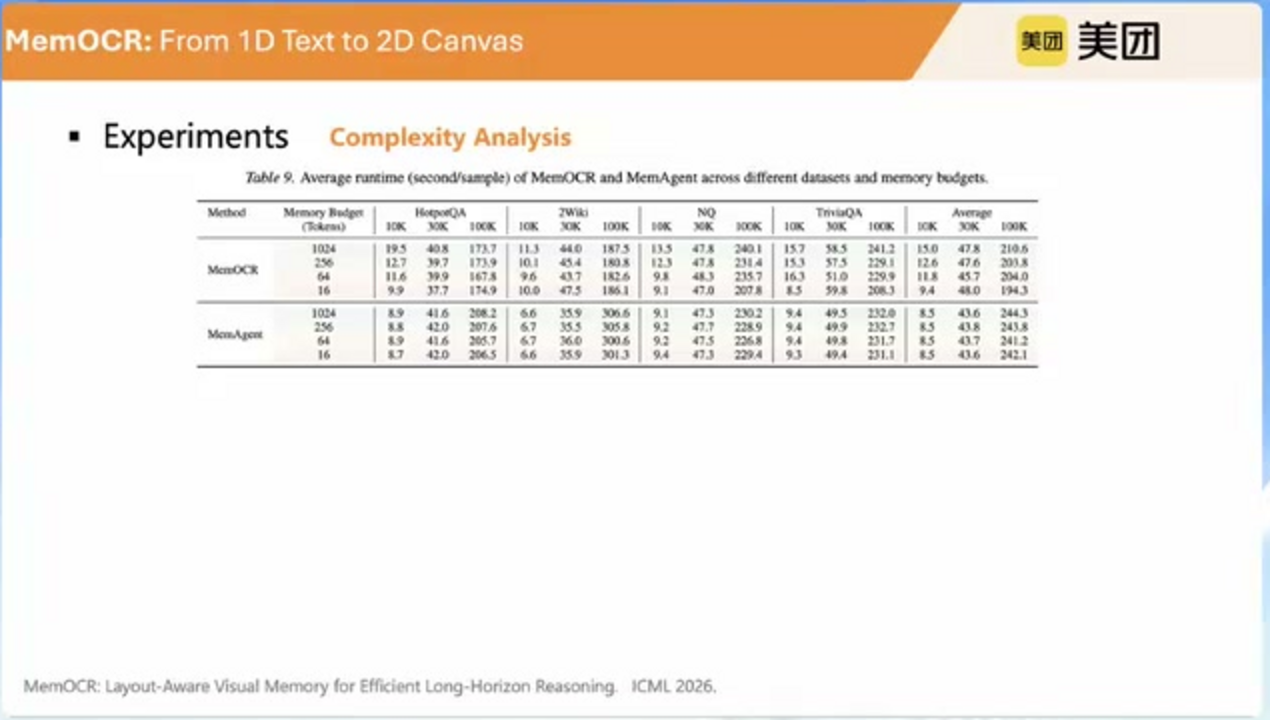
\includegraphics[width=0.86\linewidth,height=0.36\textheight,keepaspectratio]{figures/selected/fig08_complexity_analysis.png}
\caption{Complexity analysis：表格以 second/sample 统计 MemOCR 与 MemAgent 在不同数据集、上下文长度和 memory budget 下的平均运行时间。\protect\footnotemark}
\label{fig:complexity-analysis}
\end{figure}
\footnotetext{视频画面时间区间：00:17:30--00:18:00。若为裁剪图，时间区间仍对应原视频画面。}

图 \ref{fig:complexity-analysis} 里的每个数字表示处理一个 sample 需要多少秒。讲者的解释是：MemOCR 在较短上下文中会带来更明显的额外 overhead；上下文变长后，overhead 反而下降。这个现象并不神秘，因为视觉记忆可以用更少 token 表示同等信息量，字幕中提到以 512 个 token 表示同等信息量的情形。上下文越长，最终推理阶段少带一部分无关或低价值历史，收益越容易覆盖前面的渲染成本。

\begin{warningbox}{复杂度表的边界}
运行时间表只能说明当前实现、当前硬件、当前数据集上的平均 second/sample。真实部署还会受到 batch size、图片分辨率、视觉编码器实现、缓存策略、并行调度和 I/O 开销影响。若要把 MemOCR 放进生产 agent，成本评估需要重新在目标系统上测量。
\end{warningbox}

\subsection{长上下文下压缩率如何抵消开销}

压缩率的价值来自一个简单事实：回答阶段读取的信息越少，模型推理越短；前提是被保留下来的信息足够有用。文本摘要和视觉记忆都在做压缩，但它们分配压缩压力的方式不同。文本摘要常常把不同价值的信息压进同一种 token 流，视觉记忆可以通过字号、位置、层级和区域分块把压缩压力分配给不同信息。

用成本收益语言说，MemOCR 的收益是一种条件性收益：当长上下文中的低价值细节很多，而关键证据可以被可靠放入高显著区域时，视觉记忆用较小 $B$ 保留答案相关证据，最终推理时间下降。若任务需要大量细粒度数字、表格值或比较关系，压缩后的可读性会成为主风险，节省 token 的同时可能损失答案质量。

\begin{importantbox}{什么时候值得付这个成本}
MemOCR 的成本最值得支付的场景，是长上下文、多步推理、关键证据稀疏且可通过 layout 显著性保护的任务。若上下文很短，或答案依赖大量均匀细节，额外视觉流程可能缺少足够回报。
\end{importantbox}

\subsection{大模型规模与强化学习对齐的关系}

讲者还比较了未经过 RL 的更大 Qwen2.5-VL 基线。字幕中出现了 Qwen-VL 7B、32B、72B，以及“经过 RL 的 Qwen2.5-VL 7B / MemOCR”一类表述；由于中英字幕都存在机器识别噪声，模型名和具体表格数值仍应由后续 Review agent 对论文图表复核。本章只保留可由字幕稳定支持的结论：更大的未对齐基模型在平均表现上出现一定下降，在 multi-hop 这类复杂问题上差距更明显。

这个结果的含义很硬：规模增大不能自动替代任务对齐。更大的视觉语言模型也许有更强 OCR、图像理解和推理能力，但它未必知道在写 memory 时应当把哪类信息放入 crucial area，也未必经过低 memory budget 下读取显著区域的训练。MemOCR 的性能来源至少包含两个部分：

\begin{itemize}
  \item \textbf{底层能力}：视觉语言模型需要能识别压缩图像中的文字、结构和实体。
  \item \textbf{策略对齐}：训练目标需要塑造 memory drafting 和 memory reading 的协同行为，让模型知道如何分配显著性与密度。
\end{itemize}

这与人类做笔记很像。一个记忆力更强的人，如果从未学过如何做结构化笔记，可能仍会把重点、例子和边角细节混在同一页；一个训练过的人会用标题、缩进、圈注和留白表达优先级。模型规模对应“脑力”，RL 对齐对应“笔记训练”。两者互补，缺少后者时，规模很难保证 layout-aware memory policy 自然出现。

\begin{knowledgebox}{未知但重要的部署问题}
大基模对比提醒读者关注一个常被忽略的问题：MemOCR 的效果可能同时依赖训练策略和底层视觉编码器。若底层模型对小字号、密集表格、下采样中文或英文实体不稳，layout policy 再合理也会被读图能力限制。后续独立复核应特别检查不同分辨率、不同语言文字、不同表格密度下的鲁棒性。
\end{knowledgebox}

\subsection{本章小结}

本章回答“收益是否值得”的判断标准：短上下文中，MemOCR 的 renderer 和 visual memory reading 会带来明显固定成本；长上下文中，更高压缩率可以减少最终推理负担，使 overhead 下降。复杂度表支持这一趋势，但真实部署仍需按目标硬件和任务重新测量。基线比较则说明，单纯放大未经过 RL 对齐的 Qwen2.5-VL 模型不能自动复制 MemOCR 的 layout-aware 策略；有效视觉记忆需要底层识别能力，也需要 budget-aware 的训练目标。下一章应继续处理这个策略的另一面：哪些信息会在视觉压缩中最先失败。
